\documentclass[a4paper,10pt]{article}

% Packages
\usepackage[utf8]{inputenc}
\usepackage[T1]{fontenc}
\usepackage[margin=1.5cm]{geometry}
\usepackage{paracol}
\usepackage{graphicx}
\usepackage{setspace}
\usepackage{enumitem}
\usepackage{titlesec}
\usepackage{tabularx}
\usepackage{tikz}
\usepackage[most]{tcolorbox}

% Fonts ---
\usepackage{fontspec}
\setmainfont{Roboto} % Change to your preferred font


\newfontfamily\ubuntu[
    Path = ../fonts/,
    UprightFont = Ubuntu-Regular.ttf,
    BoldFont    = Ubuntu-Bold.ttf,
    ItalicFont  = Ubuntu-Italic.ttf,
    BoldItalicFont = Ubuntu-BoldItalic.ttf
]{Ubuntu}
% Fonts ---

% Section title style (uppercase, spaced)
\titleformat{\section}{\bfseries\uppercase}{\thesection}{0.5em}{}

% No numbering
\setcounter{secnumdepth}{0}

% Reduce space between items
\setlist[itemize]{nosep,left=0pt}

\begin{document}
% --- Side 1 starter her fra ---

% Header
\noindent CV / \textbf{Elias Elfarri} \hfill \textbf{Mobilutvikler} \\
\rule{\linewidth}{0.5pt}


% Space before header
\vspace{3em}

\begin{paracol}{2}
% ----- Left column -----
\begin{flushleft}
    % Profile picture
    \begin{tikzpicture}
     \clip (0,1.5) circle (2cm); % adjust size (radius)
     \node at (0,0) {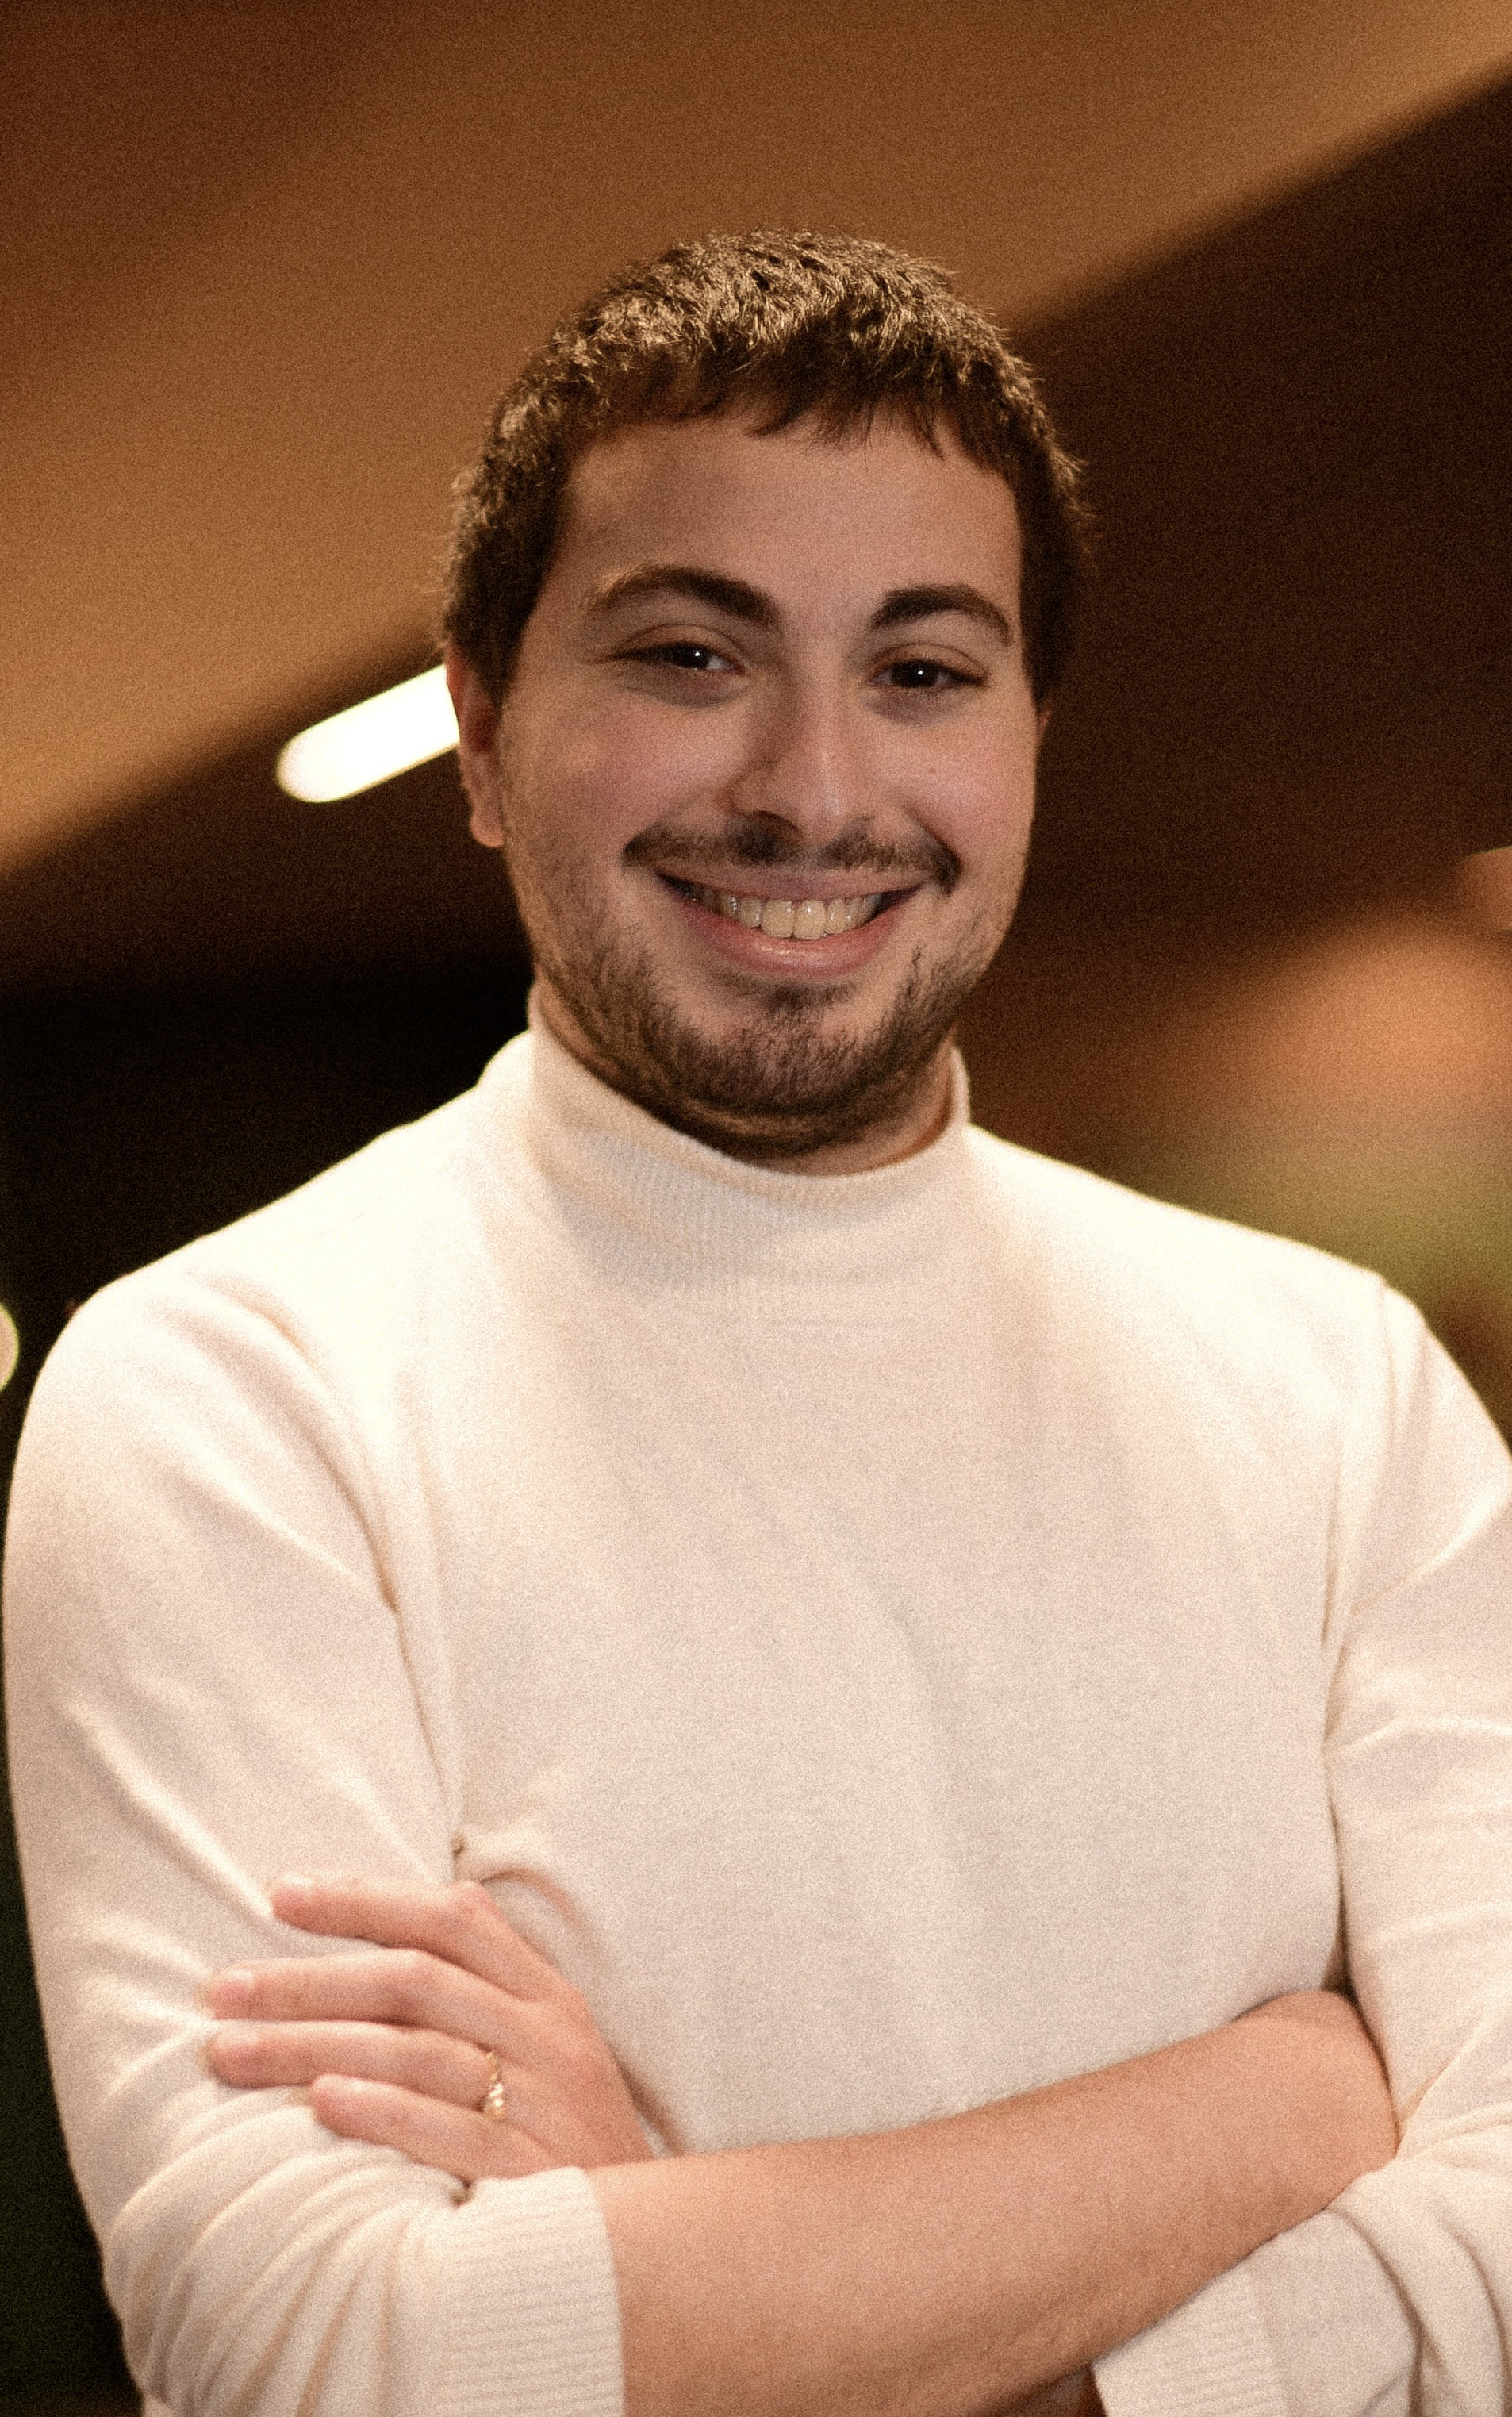
\includegraphics[width=5cm]{../portrait.jpg}};
    \end{tikzpicture}

    % a bar between image and name
    \vspace{1em}
    \noindent\rule{4cm}{10pt}
    

    \vspace{1.5em}
    {\Huge \ubuntu{Elias Elfarri}} \\
    \vspace{0.5em}
    
    \begin{tcolorbox}[
        colback=white,       % background color
        colframe=white,      % border color
        boxrule=0.0pt,       % border thickness
        arc=2mm,             % rounded corners
        width=0.85\linewidth,% make box narrower than column
        left=0mm, right=2mm, top=1mm, bottom=1mm % inner padding
        ]
    
    Elias er en mobilutvikler med 
    fire års erfaring fra både native-utvikling
     i Swift og Kotlin og kryssplattform med Flutter/Dart.
      Han har bygget opp mobilteam,
       ledet utviklingen av skalerbare
        kodebaser og publisert syv apper 
        på App Store og Google Play. 
        Med erfaring som spenner fra BLE,
         kamera og sanntids grafer til widgets 
         og spesialisert hardware-integrasjon,
          behersker han hele spekteret av
           mobilutvikling.
      Han er kjent som initiativrik, 
      reflektert og har gode pedagogiske evner.
       Elias leder Flutter Meetup-nettverket i 
       Oslo/Norge med over 500 medlemmer,
        hvor han arrangerer samlinger, 
        kurs og hackathons. 
        Dette engasjementet 
        gjør ham til en pådriver som både løfter
         prosjekter og kolleger.
    \end{tcolorbox}
\end{flushleft}

\switchcolumn

\vspace{5em}
\begin{center}
    
\end{center}
\vspace{2em}

% ----- Right column -----
 
\section{\ubuntu ERFARING}
\renewcommand{\arraystretch}{1.3} % Spacing between rows
\begin{tabularx}{\columnwidth}{@{}lX@{}}
2022 -- d.d & Fink AS, Mobilutvikler \\
2023 -- 2025 & Fink AS, Fagansvarlig Mobilutvikling \\
2021 -- 2022 & DNV, Frontend utvikler \\
2019 -- 2020 & Jenteprosjektet Ada, Prosjekt assistent \\
2018 -- 2022 & SIT, Team leder \\
2017 -- 2018 & NVFT AS, Promotør \\
2015 -- 2016 & Oslo Kommune, Hjelpepleier \\
\end{tabularx}

% space and line
\vspace{0.5em} 
\noindent\rule{\linewidth}{0.2pt}

\section{\ubuntu Utdanning}
\renewcommand{\arraystretch}{1.3} % Spacing between rows
\begin{tabularx}{\columnwidth}{@{}l>{\raggedright\arraybackslash}X@{}}
2017 -- 2022 & Norges teknisk-naturvitenskapelige universitet, Master i kybernetikk og robotikk, Sivilingeniør \\
2017 -- 2017 & Université de Caen Normandie, Utveksling \\
2016 -- 2017 & Norges teknisk-naturvitenskapelige universitet, Årsstudium i Fransk språk og litteratur \\
\end{tabularx}

% space and line
\vspace{0.5em} 
\noindent\rule{\linewidth}{0.2pt}


\section{\ubuntu Kunder}
DNV, \hspace{0.1em} 
InlineX, \hspace{0.1em} 
Norges teknisk-naturvitenskapelige
universitet

% space and line
\vspace{0.5em} 
\noindent\rule{\linewidth}{0.2pt}

\section{\ubuntu Roller}
Tech lead, \hspace{0.1em}
Mobilutvikler, \hspace{0.1em}
Frontend utvikler, \hspace{0.1em}
Fagansvarlig

\end{paracol}

\vfill
\noindent\rule{\linewidth}{0.5pt}\\
\hfill 

\newpage
% --- Side 2 starter her fra ---
% Header
\noindent CV / \textbf{Elias Elfarri} \hfill \textbf{Mobilutvikler} \\
\rule{\linewidth}{0.5pt}

  

 % TODO: add erfaringer inlinex: 2024, 2025, 2026
 % TODO: add erfaringer fra hva jeg gjorde i masteren 
 % TODO: Add Seksjon med publikasjoner, foredrag, leserinnlegg
 % TODO: Legg til tlf nr og email i headeren på første side
 % --- Verv seksjon ---
\section{Verv}
\begin{tabularx}{\linewidth}{@{}lX@{}}
2023 -- d.d & Flutter Oslo Meetup gruppe, Arrangør og leder \\
2024 -- d.d & Flutter and Friends Conference Stockholm, Arrangør \\
2018 -- 2019 & ISFiT, Dialog koordinator \\
\end{tabularx}
\vspace{1em}

% --- Stor tittel for prosjekter ---
\section{{\Huge \ubuntu PROSJEKTER}}

% --- Erfaring ---
\noindent
\begin{tabular}{@{}p{4cm}p{11cm}@{}}  % venstre = bredere, høyre = beskrivelse
\textbf{InlineX}
& \textbf{Prosjekt:} tekst kommer \\
Modningsfasen & \\
Jan.2024 - Des.2024 & \\
& \\
&  \textbf{Rolle:} \\
& \\
& \textbf{Kompetanser:} \\
\end{tabular}



\vspace{2em}

\noindent
\begin{tabular}{@{}p{4cm}p{11cm}@{}}  % venstre = bredere, høyre = beskrivelse
\textbf{InlineX}
& \textbf{Prosjekt:} I 2023 fortsatte Elias arbeidet med InlineX Mobile og tok  initiativ til å restrukturere kodebasen til et monorepo for å støtte \\
Restruktureringsfasen & utviklingen av flere enterprise nivå applikasjoner. Han utviklet blant annet Insitu Sync,  en applikasjon med robust online/offline-synkronisering,\\
Jan.2023 - Des.2023 & og bygde opp et enkelt designsystem i Figma inspirert av Material 3 og Atomic Design for gjenbruk av komponenter på tvers av web og mobil. Dette la grunnlaget for at teamet kunne levere nye produkter raskere og med høyere kvalitet. Samtidig tok Elias en nøkkelrolle i selskapets organisatoriske transformasjon. Han fikk ledelsen med på å hente inn nye roller – en ekstra utvikler, en designer og en prosjektleder (på kortere oppdrag) – noe som gjorde det mulig å etablere en mer moden produktutviklingskultur. Prosjektet markerte et vendepunkt der InlineX beveget seg fra prosjektorienterte fossefallsleveranser til å bygge en produktavdeling basert på agile prosesser, kontinuerlig discovery og tverrfaglig samarbeid.\\
& \\
& \textbf{Rolle:} Elias var både utvikler, arkitekt og endringsagent. Han tok initiativ til å etablere moderne arbeidsprosesser, fasiliterte retrospektiver og bidro aktivt til at selskapet innførte standups, sprintarbeid, OKRs, continuous discovery-trioer og stakeholder management. Han tok ansvar for å koble utvikling tettere på produkt- og forretningssiden, og sørget for at teamet hadde verktøyene og prosessene som trengtes for å skalere. \\
& \\
& \textbf{Kompetanser:} Flutter, Dart, Kotlin, Swift, Melos (monorepo), Widgetbook, Mason, Drift ORM/SQLite, RxDart, Freezed, Build Runner, Firebase Crashlytics, Azure DevOps (Git, Pipelines), VS Code, Android Studio, Xcode, Figma (Material 3, Atomic Design), Slack, Confluence, Jira, Monday, WebSockets, gRPC, stakeholder management, delivery management, OKRs, continuous discovery, fasilitering av retrospektiver, innføring av agile prosesser, produktstrategi og endringsledelse. \\
\end{tabular}


\vspace{2em}


% --- Erfaring ---
\noindent
\begin{tabular}{@{}p{4cm}p{11cm}@{}}  % venstre = bredere, høyre = beskrivelse
\textbf{InlineX}
& \textbf{Prosjekt:} Elias ble hentet inn som konsulent for å utvikle en kryssplattform applikasjon for iOS, Android og Linux, til bruk innen  energi- og\\
Startupfasen & offshore-sektoren. Oppdraget startet som en hasteløsning for kunder uten internett, men utviklet seg til å bli et strategisk produkt for \\
Aug.2022 - Des.2022 & selskapet. Elias besluttet å ta i bruk Flutter, og leverte allerede første måned en proof of concept, "InlineX Mobile", som fortsatt brukes i produksjon i dag. Løsningen ble tatt i bruk på installasjoner i blant annet Australia, Malaysia, Saudi-Arabia, Equinor Kollsnes, Nyhavna og Angola. Prosjektet markerte en av de første gangene Flutter antageligvis ble benyttet i oljebransjen.\\
& \\
& \textbf{Rolle:} Da Elias startet, bestod selskapet av kun åtte ansatte – uten etablert produktutviklingskultur, uten designer, og med kun to utviklere totalt, inklusiv Elias. Han ble derfor ikke bare mobilutvikler, men også arkitekt, strateg og pedagog. Elias hadde en sentral rolle i å forme både teknologivalg, utviklingspraksis og produktstrategi, og han konsulterte ledelsen i hvordan selskapet burde bevege seg fra ren bestillingsbasert utvikling til et moderne produkthus med egen produktavdeling. Han etablerte infrastruktur, innførte smidige utviklingsmetoder, og bygde opp grunnlaget for et bærekraftig produktmiljø. Over tid gikk han fra konsulent til å bli en nøkkelperson i selskapets teknologisatsning, med ansvar for leveranser og veiledning av andre utviklere. \\
& \\
& \textbf{Kompetanser:} Flutter, Dart, Kotlin, Swift, Android, iOS, Linux, Figma, Azure DevOps (Git, Pipelines), Firebase Crashlytics, SQLite, Riverpod, BLoC pattern, WebSockets, REST, RxDart, gRPC, KeyChain, MDM, Material Design 3, Widgetbook, Melos, Mason, Drift ORM, Shorebird, Pigeon, FFIgen, SwiftUI, Live Activities, Dynamic Island, TestFlight, Google Play Console, C++, BLE, Docker, Kubernetes, Maestro (integrasjonstesting), CI/CD, moderne produktutvikling og arkitektur. \\

\end{tabular}


\vspace{2em}

% --- Erfaring ---
\noindent
\begin{tabular}{@{}p{4cm}p{11cm}@{}}  % venstre = bredere, høyre = beskrivelse
\textbf{DNV} 
& \textbf{Prosjekt:} Elias har utviklet nye funksjoner i DP-CAP og DYN-CAP applikasjonene, brukt til beregninger og sertifisering av dynamisk pos-\\
Maritime Cybernetics Advisory & isjonering av skip. Han utviklet i Python/OpenCV basert på Watershed-metoden, som reduserte manuelt arbeid fra flere dager til sekunder, og som ble kritisk for sertifiseringsanalyser bestilt av kunder\\
2021 -- 2022 & som Equinor. Dette økte lønnsomheten av disse rapportene massivt, med en fastpris på 100 000 NOK så tok det et par klikk å levere samme analyse som kunne ta opp til en uke før. \\
& \\
& \textbf{Rolle:} Systemutvikler, backend, frontend, bildebehandlingsingeniør. \\
& \\
& \textbf{Kompetanser:} TypeScript, React, ClojureScript, Reframe, Clojure, Java, Python (OpenCV), Leiningen, Jenkins, bildebehandling/Computer Vision, PID-regulator, Watershed algoritmen og klassisk bildebehandling, PID-regulator, dynamisk posisjonering, sertifisering av DP-systemer, maritim domeneforståelse General Arrangement tegninger. \\
\end{tabular}
 


 
\end{document}